\documentclass[11pt, french, aspectratio=32]{beamer}

\usepackage{soutenance}

\AtBeginDocument{%
  \bookmark[named=FirstPage, level=subsection]{Title frame}%
}

\title{%
  Impact des Fronts sur le Phytoplancton\\
  dans la Région du Gulf Stream\\
  Quantifié par Imagerie Satellitaire
}

\author{Clément Haëck}

\direction{Marina Lévy et Laurent Bopp}

\institute{%
  Laboratoire d'Océanographie et du Climat\\Expérimentations et Analyses Numériques
}

\begin{document}

%% Title frame --------------------------

% ne pas hésiter à dire je

{
  \usebackgroundtemplate{
    \parbox[t][\paperheight]{\paperwidth}{
    \vfill\par
    \hfill
    \includegraphics[width=0.7\paperwidth, height=0.7\paperheight, keepaspectratio]{title_background.jpg}}
  }
  \begin{frame}[plain, noframenumbering]
    \titlepage%
  \end{frame}
}

\section*{Préambule}
\subsection{Le phytoplancton}

%% --------------------------------------

% -premier maillon chaîne alimentaire
% -export compensé par apport nutriment à grande échelle surtout, et complété dans les fronts fine échelle

\begingroup
\newcommand\graph[2]{%
    \llap{\includegraphics<#2>[
    height=0.85\textheight, trim=0 0 0 120, clip
    ]{_levy_2023_fig1/#1<#2>.pdf}}}%
\begin{frame}
  \frametitle{Le phytoplancton dans le système terre}
  \includegraphics[
  height=0.85\textheight, trim=0 0 0 120, clip
  ]{_levy_2023_fig1/base<1->.pdf}%
  \graph{export}{2-}%
  \graph{cycle}{3-}%
  \graph{fronts}{4-}%
  % \graph{sat}{5-}%
  % \graph{insitu}{6-}%
  % \graph{simulations}{7-}%
  \graph{frame_bot}{1-}%
\end{frame}
\endgroup

%% --------------------------------------

\subsection{Influence des courants}

% -zone d'upwelling à grande échelle
% -contrairement zone où apport plus faible

\begin{frame}
  \frametitle{Variabilité du phytoplancton: grande échelle}
  \includegraphics<1>[
    width=\textwidth, height=0.85\textheight, keepaspectratio
  ]{chl_month_avg.pdf}
  \\
  \datenote[right]{\textit{moyenne sur mai 2023, Globcolour-Copernicus}}
\end{frame}

%% --------------------------------------

\begin{frame}
  \frametitle{Variabilité du phytoplancton: (sub)mésoéchelle}
  % \begin{beamercolorbox}[sep=0pt, right]{}
    \includegraphics[height=0.8\textheight]{chl_snapshot_GS.pdf}
    \\
    \datenote[right]{\textit{L2 MODIS-Terra, 23 février 2020}}
  % \end{beamercolorbox}
\end{frame}

%% --------------------------------------

% -cas d'école

\begin{frame}
  \frametitle{Variabilité du phyplancton: front de sub-mésoéchelle}

  \includegraphics[width=0.8\textwidth]{front_exemple.pdf}
  \\
  \datenote[left]{\textit{22 avril 2007, \qtyproduct{\approx 150x150}{\km}}}

\end{frame}

%% --------------------------------------

\begin{frame}

  \boxtitle{Problématique}

  \vspace{3em}

  {
    \centering
    \begin{onehalfspacing}
      Quantifier la réponse de la chlorophylle-\textit{a}
      \\aux dynamiques de fines échelles (\(\mathcal{O}\)(10--30\,km)),
      \\dans un contexte grande échelle (\textit{ie} biorégions).
      \\
    \end{onehalfspacing}
  }
\end{frame}


\section*{Introduction}

%% --------------------------------------

% -in-situ: plusieurs mesures à différentes profondeurs

\begingroup
\NewDocumentCommand\graph{O{#3} m m}{%
    \llap{\includegraphics<#1>[
    height=0.82\textheight
    ]{_levy_2023_fig1/#2<#3>.pdf}}}%
\begin{frame}
  \frametitle{Approche: synopticité de l'imagerie satellitaire}

  \begin{columns}
    \begin{column}{0.48\textwidth}
      \includegraphics[height=0.82\textheight]{_levy_2023_fig1/base<1->.pdf}%
      \graph[1-]{export}{2-}%
      \graph[1-]{cycle}{3-}%
      \graph[1-]{fronts}{4-}%
      \graph[1-]{sat}{5-}%
      \graph[2-]{insitu}{6-}%
      \graph[3-]{simulations}{7-}%
      \graph[1-]{frame_bot}{1-}%
      \graph[1-]{frame_top}{5-}%
    \end{column}
    \begin{column}{0.50\textwidth}
      \small
      \begin{itemize}
        \item<1-> satellite:
              \begin{description}[m]
                \item[+] résolution 1km, journalière
                \item[+] \emph{synoptique}
                \item[--] en surface
              \end{description}

        \item<2-> in-situ:
              \begin{description}[m]
                \item[--] “ponctuelles”
                \item[+] résolution en profondeur
              \end{description}

        \item<3-> Modèles numériques biogéochimiques
              \begin{description}[m]
                \item[--] résolution limitée en global
              \end{description}
      \end{itemize}
    \end{column}
  \end{columns}
\end{frame}
\endgroup

%% --------------------------------------

\begingroup
\newcommand\graph[2]{%
  \llap{\includegraphics<#2>[height=0.75\textheight]{_front_circulation/#1<#2>.pdf}}}%
\begin{frame}<1-2>[label=frontogenese]
  \frametitle{Impact des fronts sur la croissance du phytoplancton}
    \includegraphics[height=0.75\textheight]{_front_circulation/base<1->.pdf}%
    \graph{upwell}{5-}%
    \graph{isopycnals}{1-}%
    \graph{jet}{2-}%
    \graph{vorticity}{3-}%
    \graph{circulation}{4-}%
    \graph{mld}{6}%
    \frametitle<6->{Impact des fronts sur la stratification}
\end{frame}

%% --------------------------------------

\begin{frame}
  \frametitle{Gulf Stream: un exemple de ‘nutrient stream’}

  \begin{itemize}
    \item Apport de nutriments à grande échelle par le Gulf Stream
  \end{itemize}
  \begin{block}{}
    \includegraphics[width=0.65\textwidth]{whitt_2019.pdf}
    {\hspace{1em}\footnotesize\textit{\raisebox{2em}{Whitt 2019}}}
  \end{block}
\end{frame}

%% --------------------------------------

\againframe<3-5>{frontogenese}

%% --------------------------------------

\begin{frame}
  \frametitle{Quantification}
  \begin{columns}
    \begin{column}{0.66\linewidth}
      \begin{itemize}
        \item Variabilité spatio-temporelle de la Chl-a (satellite) en Océan Austral
              \\
              {\footnotesize\textit{Prend et al. 2022, Keerthi et al. 2022}}
      \end{itemize}
    \end{column}
    \begin{column}{0.33\linewidth}
      \includegraphics[width=\linewidth]{levy_2023_fig3.pdf}
    \end{column}
  \end{columns}

  \vspace*{2em}

  \visible<2->{
  \begin{columns}
    \begin{column}{0.5\linewidth}
      \begin{itemize}
        \item Impact des fronts de SST sur Chl-a (Gyre Subtropicale du Pacifique Nord)
              \\
              {\footnotesize\textit{Liu \& Levine 2016}}
      \end{itemize}
    \end{column}
    \begin{column}{0.5\linewidth}
      \includegraphics[height=0.45\textheight]{liu_levine.png}
    \end{column}
  \end{columns}
  }
\end{frame}

%% --------------------------------------

\againframe<6>{frontogenese}
\endgroup

%% --------------------------------------

\begin{frame}
  \frametitle{Modification de la phénologie du bloom}

  \begin{block}{}
    Modèle numérique biogéochimique régional
    \begin{itemize}
      \item run avec fronts (en noir)
            \\\(\rightarrow\) correspond aux observations (\textcolor{red}{en rouge})
      \item<2-> run sans fronts (\textcolor{violet}{en violet})
            \\\(\rightarrow\) bloom tardif (\qty{\approx 30}{\text{jours}})
    \end{itemize}
  \end{block}

  \includegraphics[width=0.5\textwidth]{mahadevan_2012_fig3.pdf}
  {\hspace{1em}\footnotesize\textit{\raisebox{2em}{Mahadevan et al.\ 2012}}}
\end{frame}

%% --------------------------------------

\section{Objectifs}

\begin{frame}
  \boxtitle{Objectifs}
  \vspace{2em}

  \begin{beamercolorbox}[sep=0pt]{}
    \begin{enumerate}
      \setlength{\itemsep}{1.2em}
      \item Quantifier la \emph{réponse de la chlorophylle-a} aux dynamiques \emph{frontales}
      \item<2-> Influence de la \emph{saison}, du \emph{régime} biogéochimique, et du \emph{type} de fronts ?
      \item<3-> Détecter un \emph{bloom précoce} dans les fronts ?
    \end{enumerate}
  \end{beamercolorbox}
\end{frame}

%% --------------------------------------

% -anomalie chaude = Gulf Stream
% -correspond à délimitation biorégions
% -plan de l'exposé, détailler point par point

\begingroup
\newcommand\graph[2]{%
    \llap{\includegraphics<#2>[
    width=\textwidth, height=0.9\textheight, keepaspectratio
    ]{_region_etude/#1<#2>.pdf}}}%
\begin{frame}
  \frametitle{Région d'étude: autour du Gulf Stream}
  \includegraphics[
  width=\textwidth, height=\textheight, keepaspectratio
  ]{_region_etude/base_chl<1->.pdf}%
  \graph{base_sst}{1-7}%
  \graph{gulfstream}{2-7}%
  \graph{gyre}{3-7}%
  \graph{talus}{4-7}%
  \graph{subtrop_perm}{5-}%
  \graph{subpol}{6-}%
  \graph{subtrop_sais}{7-}%
  \graph{problematiques}{8-}%
  \frametitle<8->{Plan}

  \datenote[right]{moyennes sur mai 2023}
\end{frame}
\endgroup

%% --------------------------------------

\section*{Méthodes - Détection des fronts}

\begin{frame}
  \boxtitle{Méthodes - Détection des fronts}
\end{frame}

%% --------------------------------------

% -structures résolues à 4km et +léger

\begin{frame}
  \frametitle{Données utilisées: Chl-a}

  \begin{block}{}
    \begin{itemize}
      \item Copernicus-Globcolour,
      \item journalières, 4km, 2000--2020
      \item L3: multicapteurs, avec nuages
    \end{itemize}
  \end{block}

  \vfill

  {\footnotesize\textit{\raisebox{2em}{22 avril 2007}}}
  \includegraphics[height=0.5\textheight]{comparaison_chl.pdf}%
\end{frame}

%% --------------------------------------

% -même résolution que Chl
% -Glorys: structures frontales ne sont pas positionnés aux bons endroits (décalages)

\begin{frame}
  \frametitle{Données utilisées: SST}

  \begin{block}{}
    \begin{itemize}
      \item proxy de la densité
      \item ESA-SST-CCI / C3S
      \item journalières, 4km, 2000--2020
      \item L4: interpolation spatiale de multicapteurs IR, pas de nuages
    \end{itemize}
  \end{block}

  \vfill

  {\footnotesize\textit{\raisebox{2em}{22 avril 2007}}}
  \includegraphics[height=0.5\textheight]{comparaison_sst.pdf}%

\end{frame}

%% --------------------------------------

\begin{frame}
  \frametitle{Détecter les fronts par satellite}

  \begin{columns}[t]
    \begin{column}{0.45\textwidth}
      \begin{itemize}
        \item détection d'une \emph{frontière}:
      \end{itemize}

      \begin{center}
        \includegraphics[width=0.7\linewidth]{nieto_2012.pdf}

        \vspace{0.5em}

        Canny, Cayula--Cornillon, \textsb<1>{Nieto}, Miller, \ldots
      \end{center}
    \end{column}

    \visible<2->{
    \begin{column}{0.55\textwidth}
      \begin{itemize}
        \item détection d'une \emph{zone frontale}:
      \end{itemize}

      \begin{center}
        \includegraphics[width=\linewidth]{front_exemple_zone.pdf}

        \vspace{0.5em}

        Belkin--O'Reilly, \emph{Liu \& Levine 2016}
      \end{center}
    \end{column}}
  \end{columns}
\end{frame}

%% --------------------------------------

% -on voit à l'oeil nu qu'un seuil à 5 permet de bien délimiter

\begingroup
\newcommand\graphstep[2]{%
  \llap{\includegraphics<#2>[width=\textwidth]{_composantes/#1<#2>.pdf}}}%
\begin{frame}
  \frametitle{Détection des fronts: méthode du “Heterogeneity-Index” (HI)}

  \begin{itemize}
    \item Application d'une fenêtre glissante sur SST
          % (taille \qtyrange{10}{30}{\km})
  \end{itemize}

  \vfill

  \includegraphics[width=\textwidth]{_composantes/base<1->.pdf}%
  \graphstep{composantes}{2-3}%
  \graphstep{chla}{1,4-}%
  \graphstep{HI}{2-}%
  \graphstep{contours}{3-}%
  \graphstep{contours_compo}{3}%
  \graphstep{contours_sst}{4-}%
\end{frame}
\endgroup

%% --------------------------------------

\begin{frame}
  \frametitle{Évolution de la chl-a avec le HI}
  \includegraphics[
  width=\textwidth, height=0.8\textheight, keepaspectratio
  ]{results/chl_vs_hi.pdf}
  \\
  \datenote[right]{sur 2000-2020}
\end{frame}

%% --------------------------------------

% -j'ai choisi 2 seuils qui donnent répartition suivante:

\begingroup
\newcommand\graph[2]{%
  \llap{\includegraphics<#2>[height=0.8\textheight]{results/_fronts_occurrence/#1<#2>.pdf}}}%
\begin{frame}
  \frametitle{Cartes de probabilité de présence des fronts}
  \includegraphics[height=0.8\textheight]{results/_fronts_occurrence/base<1->.pdf}%
  \graph{delineation}{1-2}%
  \graph{maps}{2-}%
  \graph{fronts}{3-}%

\end{frame}
\endgroup

%% --------------------------------------

\section{Région subtropicale -- Augmentation de la Chlorophylle dans les fronts}
\begingroup
\newcommand\graph[1]{%
    \llap{\includegraphics[
    width=\textwidth, height=0.9\textheight, keepaspectratio
    ]{_region_etude/#1.pdf}}}%
\begin{frame}
  \boxtitle{Partie 1}

  \includegraphics[
  width=\textwidth, height=\textheight, keepaspectratio
  ]{_region_etude/base_chl<1->.pdf}%
  \graph{subtrop_perm<5->}%
  \graph{subtrop_sais<7->}%
  \graph{subpol<6->}%
  \graph{problematiques<8->}%
  \graph{blocker_2}%
  \graph{blocker_3}%
\end{frame}
\endgroup

%% --------------------------------------

\begingroup
\newcommand\graphstep[2]{%
  \llap{\includegraphics<#2>[
    width=\textwidth, height=0.8\textheight, keepaspectratio
    ]{_distrib_region_perm/#1<#2>.pdf}}}%
\begin{frame}
  \frametitle{Mesure de l'impact des fronts}
  \includegraphics[
    width=\textwidth, height=0.8\textheight, keepaspectratio
  ]{_distrib_region_perm/base<1->.pdf}%
  \graphstep{histogram}{2-}%
  \graphstep{medianes}{3-}%
  \graphstep{latband}{4-}%
\end{frame}
\endgroup

%% --------------------------------------

\begingroup
\newcommand\graphstep[2]{%
  \llap{\includegraphics<#2>[height=0.8\textheight]{_res_perm/#1<#2>.pdf}}}%
\begin{frame}
  \frametitle{Augmentation locale de la chl-a}
  \includegraphics[height=0.8\textheight]{_res_perm/base<1->.pdf}%
  \graphstep{med_one_year}{1}%
  \graphstep{histogram}{1}%
  \graphstep{med_all_years}{2}%
  \graphstep{med_cli}{3-}%
  \graphstep{exces}{4-}%
  \graphstep{comparaison}{5-}%

  \datenote{dans la bande 25--30°N}
\end{frame}
\endgroup

%% --------------------------------------

\begin{frame}
  \frametitle{Comparaison avec l'estimation de Liu \& Levine (2016)}
  \begin{columns}[t]
    \begin{column}{0.48\textwidth}
      \begin{itemize}
        \item taille de la fenêtre glissante (10km vs 30km) ?
      \end{itemize}
      \visible<2->{
        \begin{center}
          \includegraphics[height=3cm]{ts_sensitivity.pdf}
          \\
          excès peu sensibles à la taille (\pct{<15} de variation)
        \end{center}
      }
    \end{column}

    \begin{column}{0.48\textwidth}
      \begin{itemize}
        \item Correction du biais de grande échelle ?
      \end{itemize}

      \visible<3->{
        \begin{center}
          \includegraphics[height=4cm]{biais_gradient.pdf}
          \\
          surestimation si non corrigé
        \end{center}
      }
    \end{column}
  \end{columns}
\end{frame}

%% --------------------------------------

% -exces pas suffisant
% -il faut tenir compte de la surface des fronts

\begin{frame}
  \frametitle{Effet régional sur la chl-a}

  \begin{itemize}
    \item Tenir compte de la surface des fronts
  \end{itemize}

  \includegraphics[width=\textwidth]{_surplus/base<1->.pdf}%
  \llap{\includegraphics<2->[width=\textwidth]{_surplus/surplus<2->.pdf}}%

  \vfill

  \visible<2->{
  \begin{itemize}
    \item effet des fronts très faible à l'échelle régionale
  \end{itemize}}
\end{frame}

%% --------------------------------------

\begin{frame}
  \frametitle{Conclusion partie 1}
  \begin{minipage}{0.85\linewidth}
    \begin{itemize}
            \setlength{\itemsep}{3em}
      \item augmentation locale de la Chl-a~(\pct{\approx 10})
            \begin{itemize}
              \item[$\longrightarrow$] apport vertical de nutriments par les fronts
            \end{itemize}
      \item important de corriger biais de grande échelle
      \item effet régional faible si la surface des fronts prise en compte~(\pct{\approx 3})
    \end{itemize}
  \end{minipage}
\end{frame}

%% --------------------------------------

\section{Région du Gulf-Stream -- Intensité des fronts}
\begingroup
\newcommand\graph[1]{%
    \llap{\includegraphics[
    width=\textwidth, height=0.9\textheight, keepaspectratio
    ]{_region_etude/#1.pdf}}}%
\begin{frame}
  \boxtitle{Partie 2}

  \includegraphics[
  width=\textwidth, height=\textheight, keepaspectratio
  ]{_region_etude/base_chl<1->.pdf}%
  \graph{subtrop_perm<5->}%
  \graph{subtrop_sais<7->}%
  \graph{subpol<6->}%
  \graph{problematiques<8->}%
  \graph{blocker_1}%
  \graph{blocker_3}%
\end{frame}
\endgroup

%% --------------------------------------

\begingroup
\newcommand\graph[2]{%
  \llap{\includegraphics<#2>[
    width=\textwidth, height=0.8\textheight, keepaspectratio
    ]{_zone_separation/#1<#2>.pdf}}}%
\begin{frame}
  \frametitle{Détection journalière du mur nord du Gulf Stream}
  \includegraphics[
  width=\textwidth, height=0.8\textheight, keepaspectratio
  ]{_zone_separation/base<1->.pdf}%
  \graph{distrib_IN}{1-2}%
  \graph{fit}{2}%
  \graph{threshold}{3-}%
  \graph{selection}{4-}%
  \graph{base_top}{1-}%

  \datenote[left]{23 février 2020}
\end{frame}
\endgroup

%% --------------------------------------

\begingroup
\newcommand\graph[2]{%
  \llap{\includegraphics<#2>[width=\textwidth]{_res_sais_exces/#1<#2>.pdf}}}%
\begin{frame}
  \frametitle{Impact des fronts (faibles et forts) sur la Chl-a}
  \includegraphics[width=\textwidth]{_res_sais_exces/base<1->.pdf}%
  \graph{exces}{2-}%

  \vfill

  \begin{itemize}
    \item Effet local beaucoup plus important dans les \textcolor{plotfort}{fronts forts}
  \end{itemize}

  \begin{itemize}
          \setlength{\itemindent}{2em}
    \item<3->[$\longrightarrow$] impact du ‘nutrient stream’
    \item<3->[$\longrightarrow$] circulations plus profondes
  \end{itemize}
\end{frame}
\endgroup

%% --------------------------------------

\begingroup
\newcommand\graph[2]{%
  \llap{\includegraphics<#2>[width=\textwidth]{_res_sais_surplus/#1<#2>.pdf}}}%
\begin{frame}
  \frametitle{Impact des fronts (faibles et forts) sur la Chl-a}
  \includegraphics[width=\textwidth]{_res_sais_surplus/base<1->.pdf}%
  \graph{surplus}{2-}%

  \vfill

  \begin{itemize}
    \item Les fronts forts occupent moins de \emph{surface}
    \item<2-> Effet régional \emph{comparable} pour les fronts forts et faibles
  \end{itemize}
\end{frame}
\endgroup

%% --------------------------------------

\begin{frame}
  \frametitle{Conclusion partie 2}

  \vfill
  \begin{itemize}
    \setlength{\itemsep}{1em}
    \item augmentation de chl-a beaucoup plus importante dans les fronts forts
          \begin{itemize}
            \item[$\longrightarrow$] circulation plus profonde
            \item[$\longrightarrow$] nutrient stream
          \end{itemize}
    \item effet à l'échelle régionale comparable entre fronts forts et faibles
  \end{itemize}
  \vfill

\end{frame}

%% --------------------------------------

\section{Région subpolaire -- Phénologie du bloom}
\begingroup
\newcommand\graph[1]{%
    \llap{\includegraphics[
    width=\textwidth, height=0.9\textheight, keepaspectratio
    ]{_region_etude/#1.pdf}}}%
\begin{frame}
  \boxtitle{Partie 3}

  \includegraphics[
  width=\textwidth, height=\textheight, keepaspectratio
  ]{_region_etude/base_chl<1->.pdf}%
  \graph{subtrop_perm<5->}%
  \graph{subtrop_sais<7->}%
  \graph{subpol<6->}%
  \graph{problematiques<8->}%
  \graph{blocker_1}%
  \graph{blocker_2}%
\end{frame}
\endgroup

%% --------------------------------------


\begingroup
\newcommand\graph[2]{%
    \llap{\includegraphics<#2>[
    width=\textwidth, height=0.8\textheight, keepaspectratio
    ]{_phenologie_méthode/#1<#2>.pdf}}}%
\begin{frame}
  \frametitle{Chronométrer le bloom: démarrage et durée}
  \includegraphics[
    width=\textwidth, height=0.8\textheight, keepaspectratio
  ]{_phenologie_méthode/base<1->.pdf}%
  \graph{dchl_base}{4-}%
  \graph{dchl}{4}%
  \graph{xlabels_top}{2,3}%
  \graph{chl_daily}{2-}%
  \graph{chl_filtre}{3-}%
  \graph{step_max}{5-}%
  \graph{onset}{6-}%
  \graph{onset_short}{6}%
  \graph{onset_uncertainty}{7-}%
  \graph{fin_bloom}{8-}%
  \graph{fin_bloom_short}{8}%
  \graph{fin_uncertainty}{9-}%
  \graph{dchl_axes_top}{4-}%
  \graph{axes_top}{2-}%
  \graph{chl}{1-3}%
  \graph{pointer}{2,3}%
\end{frame}
\endgroup

%% --------------------------------------

\begin{frame}
  \frametitle{Différences de phénologie entre background et fronts}
  \multigraph[width=\textwidth, height=0.8\textheight, keepaspectratio]{4}{phenologie_lag}
\end{frame}

%% --------------------------------------

\begingroup
\newcommand\graph[2]{%
  \llap{\includegraphics<#2>[height=0.7\textheight]{_bloom/#1<#2>.pdf}}}%
\begin{frame}
  \frametitle{Décalage du \emph{\textit{démarrage}} du bloom}
  \includegraphics[height=0.7\textheight]{_bloom/base<1->.pdf}%
  \graph{blue_error}{2-}%
  \graph{cyan_error}{3-}%
  \graph{orange_error}{4-}%
  \graph{green_error}{5-}%
  \graph{blue_scatter}{2-}%
  \graph{cyan_scatter}{3-}%
  \graph{orange_scatter}{4-}%
  \graph{green_scatter}{5-}%
  \graph{fit_faible}{6-}%
  \graph{fit_fort}{7-}%
  \graph{base_top}{1-}%

  \vfill

  \begin{overlayarea}{\textwidth}{2\baselineskip}
    \only<6->{fit pour les fronts faibles: \(-6.7 \pm 1.1\) jours}

    \only<7->{fit pour les fronts forts: \(-13.5 \pm 1.5\) jours}
  \end{overlayarea}
\end{frame}
\endgroup

%% --------------------------------------

\begin{frame}
  \frametitle{Décalage de la \emph{\textit{durée}} du bloom}
  \includegraphics[
  width=0.90\textwidth, height=0.7\textheight,
  keepaspectratio]{durée_bloom.pdf}

  \vfill

  Blooms plus \emph{longs} dans les \emph{fronts}, mais moins significatif
\end{frame}

%% --------------------------------------

\begin{frame}
  \frametitle{Conclusion partie 3}
  \vfill
  \begin{itemize}
          \setlength{\itemsep}{3em}
    \item détection d'une avance du bloom dans les \emph{fronts} d'une à deux semaines
          \begin{itemize}
            \item[$\longrightarrow$] effet des fronts sur la stratification
          \end{itemize}
    \item pas d'effet significatif sur la durée du bloom
  \end{itemize}
  \vfill
\end{frame}

%% --------------------------------------

\section{Conclusions}

\begin{frame}
  \boxtitle{Conclusions}

  \vspace{\stretch{2}}

  \begin{itemize}
          \setlength{\itemsep}{0.8em}
    \item Quantification à l'échelle régionale de l'effet des fines échelles
    \item Effet plus important dans la région subpolaire
          % \begin{itemize}
          %   \item nutricline moins profonde
          %   \item nutrient stream
          % \end{itemize}
  \end{itemize}

  \vspace{\stretch{1}}

  \includegraphics[height=0.6\textheight]{article_review.pdf}

  \vspace{\stretch{1}}
\end{frame}

\section{Perspectives}

%% --------------------------------------

\begin{frame}
  \frametitle{Perspectives: Application à la composition du phytoplancton}

  \begin{itemize}
    \item cartes de concentration par groupe fonctionnel (PFT) obtenues par SOM (El Hourany et al. 2019)
  \end{itemize}

  \vfill
  \includegraphics[width=0.75\textwidth]{ts_pft.pdf}
  \vfill

  \begin{itemize}
    \item[$\longrightarrow$] réponse différente selon le groupe
  \end{itemize}
\end{frame}

%% --------------------------------------

\begin{frame}
  \frametitle{Perspectives: Application à l'échelle globale}

  \includegraphics[height=0.7\textheight]{global_hi.pdf}

  \begin{itemize}
    \item difficultés techniques: cette image = \qty{60}{\MO}
          \\{\small(\mbox{20 ans = \qty{0.5}{\TO}} pour le HI seul)}
  \end{itemize}

\end{frame}

%% --------------------------------------

\begin{frame}
  \frametitle{Perspectives: outils pour la quantification des effets des fronts}

  \begin{itemize}
    \item quantification haute résolution sur grande surface
    \item[$\lightning$] analyses complexes, exploratoires / itératives
  \end{itemize}
  {\usebeamercolor[fg]{structure}\(\Rightarrow\)} nécessité d'outils adaptés
  \vfill

  \visible<2->{
  \begin{itemize}
    \item \num{11 000} lignes de codes + documentation
          \\{\scriptsize (\url{https://gitlab.in2p3.fr/clement.haeck/submeso-color})}
    \item packets python génériques:
          \href{https://pypi.org/project/filefinder/}{{\footnotesize PyPi}:filefinder},
          \href{https://pypi.org/project/tol-colors/}{{\footnotesize PyPi}:tol-colors}
    \item participation à
          \href{https://github.com/xarray-contrib/cf-xarray/pull/354}{cf-xarray}
  \end{itemize}
  }

  \vfill

  \visible<3->{{\usebeamercolor[fg]{structure}\(\Rightarrow\)} Continuer à rendre plus facilement utilisable
  \\pour d'autres utilisateurs}

\end{frame}

\appendix


\end{document}
